\documentclass[11pt,a4paper]{article}
\usepackage[margin=1in]{geometry}
\usepackage{booktabs}
\usepackage{graphicx}
\usepackage{hyperref}
\usepackage{float}
\usepackage{caption}
\usepackage{setspace}
\usepackage{amsmath}
\usepackage{amssymb}
\setstretch{1.1}
\graphicspath{{figures/}}

\title{AI651 Assignment 2 Report}
\author{Muhammad Tayyab Tahir Qureshi\\Roll number 25280024\\Lahore University of Management Sciences}
\date{Fall 2026}

\begin{document}
\maketitle

\noindent\textbf{Name:} Muhammad Tayyab Tahir Qureshi\\
\noindent\textbf{Roll number:} 25280024\\
\noindent\textbf{GitHub repository (public):} \url{https://github.com/ttqureshi/DL4STG-PA2}

\section{Question 1}

\subsection{Architecture diagram}

One model forecasts the water level at S1--S4. Eight series are aligned on a 10-minute clock: levels at S1, S2, S3, S4, and T1, rainfall at R1 and R2, and the reservoir release. They are projected into tokens, mixed by two attention blocks, and read out as six future levels at each station. The river is not placed on a grid. With a 6-hour history (A1) and a six-step horizon (A2), \(L = 8\times 36 + 6 = 294\) tokens and width \(d = 64\). Those sizes are design choices, not facts from the brief.

A station's own history is not enough. Two issuances can share S2's 36 levels and differ at S1 or T1. A stack that only reads S2 must return the same forecast for both. The token list contains the other series, so the two issuances are different inputs.

Reach is set by the mixer. One attention block connects every unmasked token to every other. A second block does not see farther; it can use a combination the first block has already formed. Stations are unevenly spaced, so I do not count reach in hops. A local mixer that saw only the immediate upstream station would need many blocks before S4 could see the reservoir. Attention buys that path in one block. A path is not the same as the model using it. The S4 query can put its weight on its own recent tokens, or near the uniform weight \(1/294\), and the learned upstream bias can go to zero.

Attention is cheap here because there are eight series. One block costs about \(2L^{2}d \approx 1.1\times 10^{7}\) multiply-adds. A \(64\times 64\) field over the same 36 times would be on the order of \(10^{5}\) times larger. The 10-minute cycle is limited by when the gauges arrive, not by this forward pass. That count is from the shapes. It is not a measured runtime.

\begin{verbatim}
Issuance t.  Delta = 10 min.  H = 36 (A1).  F = 6 leads (A2).
Levels S1--S4, T1     (B, 5, H) value and mask     -> (B, 5, H, d)
Rain R1, R2           (B, 2, H) value and mask     -> (B, 2, H, d)
Release history       (B, 1, H) actual, schedule, mask
Announced future      (B, 1, F) schedule and known mask
Flatten and concatenate: L = 8H + F = 294.  Z0 is (B, L, d).
Two attention blocks -> Z2 (B, L, d).
Readout: 4 x 6 = 24 queries.  Forecast Yhat is (B, 4, 6).
\end{verbatim}

History bins are \(t-(H-1)\Delta,\ldots,t\). Horizon bins are \(t+\Delta,\ldots,t+F\Delta\). Rain is binned onto the level clock. Releases are held constant between effective times. Future rain and future levels are not tokens. Masked history tokens stay in the list so \(L\) is fixed, and their attention score is \(-\infty\).

\subsection{Assumptions}

The following are given. The reservoir releases into the main river upstream of S1. Monitored tributary T1 joins between S1 and S2. An unmonitored tributary joins between S2 and S3. Stations are unevenly spaced and travel times change. Levels at S1--S4 and T1 are recorded every ten minutes. Rainfall at R1 and R2 comes with timestamps and locations. Recorded releases and schedules already announced at issuance come with announcement and effective times. Locations, connectivity, and distances are available. Precise travel times, unmonitored inflows, future rainfall, and future levels are not.

The brief does not state a history length, whether ``one hour ahead'' is one level or the path inside the hour, the record length, the reporting delay, the noise, or that rain shares the level clock.

\begin{itemize}
\item \textbf{A1.} History is \(H=36\) bins, six hours, ending at issuance. Six hours is several times the horizon and keeps \(L\) near 300. A longer travel time is invisible except through the level it has already produced.
\item \textbf{A2.} The output is six levels at each of S1--S4, at \(+10\) through \(+60\) minutes. The service names the hour-ahead level; the path is what a flood desk uses. This sets \(\hat Y\) to shape \((B,4,6)\).
\item \textbf{A3.} The archive covers at least one year, including wet and dry periods. Inference reads only the window in A1.
\item \textbf{A4.} On a normal issuance the bin that closes at \(t\) has arrived. When it has not, the bin stays masked and the forecast still goes out.
\item \textbf{A5.} Gauge errors are small beside a rise that matters. There is no separate denoiser. A stuck gauge would be learned as if it were the river.
\item \textbf{A6.} Each rain reading is placed in the 10-minute bin that contains its timestamp. An empty bin repeats the last reading and is marked carried. Carried bins get no attention weight.
\item \textbf{A7.} Releases are piecewise constant between effective times. If several announcements for one effective time are already public, the latest is used.
\item \textbf{A8.} S1--S4 and T1 share 10-minute boundaries, so one lag index is the same time at every station.
\item \textbf{A9.} Water moves downstream. Travel time is not distance over a constant speed. Past downstream levels remain legal inputs.
\item \textbf{A10.} The target is level. Each series is standardized with its training mean and standard deviation, and that scale is inverted before the number is issued.
\item \textbf{A11.} R1 and R2 are not assigned to reaches. Both are tokens, and gauge-to-station distance is a feature.
\item \textbf{A12.} The unmonitored tributary has no gauge. The S3 minus S2 residual, masked if either level is missing, is an extra channel on the history. It is zero on the other series.
\item \textbf{A13.} Future rainfall and future levels are not inputs. A future release is written only when its announcement time is at or before issuance.
\item \textbf{A14.} Training uses the same clock. Inputs at issuance \(t\) obey A13, and the target is the level later recorded at \(t+\Delta,\ldots,t+6\Delta\).
\item \textbf{A15.} The loss is mean squared error of the standardized level, averaged over stations, leads, and the batch. Missing targets are left out. The issued number is a point forecast, not a flood probability.
\item \textbf{A16.} Along-river distances are used among the reservoir, S1--S4, and T1. Gauge-to-station distance is straight-line. Neither is turned into a travel time.
\end{itemize}

\subsection{Task and data table}

An issuance is computed when a 10-minute bin closes. Call that time \(t\). The history is the \(H=36\) bins from \(t-35\Delta\) to \(t\). The horizon is leads \(h=1,\ldots,6\) at \(t+h\Delta\). Outputs are the six future levels at S1--S4. T1 is an input, not a target. In operation the batch size is 1.

\begin{table}[H]
\centering
\caption{Inputs and the forecast at issuance \(t\). Shapes are after alignment and before the width-\(d\) projection. Masks are in \(\{0,1\}\).}
\small
\begin{tabular}{llll}
\toprule
Name & Shape & Time & At issuance \\
\midrule
Level history & \((B,5,H)\) & \(t-(H-1)\Delta\ldots t\) & Known \\
Level mask & \((B,5,H)\) & same bins & Known \\
S3\(-\)S2 residual & \((B,5,H)\) & same; 0 if either missing & Constructed \\
Rain, aligned & \((B,2,H)\) & level-clock bins & Past only \\
Rain mask & \((B,2,H)\) & 1 if a real reading & Known \\
Actual release & \((B,1,H)\) & bins ending at \(t\) & Known \\
Schedule on history & \((B,1,H)\) & already public & Known \\
Future release & \((B,1,F)\) & \(t+\Delta\ldots t+6\Delta\) & If announced by \(t\) \\
Future-release mask & \((B,1,F)\) & 1 if public & Known \\
Upstream \(U\), distances & \((8,8)\) & static & Known \\
Forecast \(\hat Y\) & \((B,4,6)\) & \(t+\Delta\ldots t+6\Delta\) & Target, never an input \\
\bottomrule
\end{tabular}
\end{table}

Series order is S1, S2, S3, S4, T1, R1, R2, release. Tokens that share a lag index refer to the same 10-minute bin. Future release tokens use the lead index, so a horizon bin is not stored as a past observation. At issuance the model may see every row except \(\hat Y\), and the future-release row only through announcements already public.

\subsection{Notation, equations, and objective}

\(\Delta = 10\) minutes. Lag \(\ell = 0,\ldots,H-1\) means time \(t-\ell\Delta\). Lead \(h=1,\ldots,6\) means time \(t+h\Delta\). \(U_{j,i}=1\) when series \(j\) is upstream of series \(i\). Into S1: the release only. Into S2: the release, S1, and T1. Into S3: those plus S2. Into S4: those plus S3. A station is not upstream of itself. \(\phi(d)=-\log(1+d/d_0)\), with \(d_0\) the median static distance. \(\lambda_{\mathrm{up}}\) and \(\lambda_{\mathrm{dist}}\) are learned scalars.

A level token carries the standardized level, the mask, and the residual channel. Rain carries standardized rain and its mask. A history release carries actual, schedule, and the actual mask. A future release carries the announced value and the known mask. Each group has its own matrix,
\[
e = W_{\mathrm{group}} x + a_i + b_{\mathrm{time}},
\]
and the token list is \(Z^{(0)}\in\mathbb{R}^{L\times d}\). For block \(n=1,2\),
\[
\mathrm{score}(p,q) = \frac{Q_p\cdot K_q}{\sqrt{d}} + \lambda_{\mathrm{up}} U_{\mathrm{series}(q),\mathrm{series}(p)} + \lambda_{\mathrm{dist}}\phi(d_{q,p}).
\]
A key whose mask is 0 has score \(-\infty\). The block is residual attention plus a residual feed-forward layer of width \(4d\). The query for lead \(h\) at station \(s\) is \(q_{s,h} = W_q[z_{s,0}; e_h; \tau_s]\), where \(\tau_s\) is how many bins since \(s\) last reported. The loss, with \(m_{s,h}(t)=1\) when the target was recorded, is the mean over the batch of
\[
\frac{\sum_{s,h} m_{s,h}(\hat y^{\mathrm{std}}_{s,h}-y^{\mathrm{std}}_{s,h})^{2}}{\sum_{s,h} m_{s,h}}.
\]
Separate projections exist because the units differ. One token list exists so S2 can see S1 and T1. Lead-specific queries let \(+10\) and \(+60\) minutes weight different lags. The head is direct, not a rollout that writes predicted levels back as if they had been measured. What is fixed is the series list, \(U\), the ban on future rain and future levels, and the rule that an announcement enters only if it is already public. What is learned is every matrix, both blocks, the readout, and the four bias scalars. A route in the wiring is not evidence that the weights use it.

\subsection{Operation}

\textbf{Missing observations.} A missing value is set to 0 after standardization and its mask to 0. The token stays, so \(L\) does not change, and the score rule gives it no weight. The residual is masked if either of S2 or S3 is missing. A missing S1 does not block the S4 forecast.

\textbf{Delayed observations.} A bin that has not arrived by \(t\) is missing. The readout also sees \(\tau_s\), the bins since that station last reported. The forecast is issued on the 10-minute mark. It does not wait for a late packet. The next issuance, ten minutes later, can fill the earlier bin if the packet has arrived.

\textbf{Announced future releases.} For each lead, the latest announcement with announcement time at or before \(t\) and effective time in that bin is the value, and the known mask is 1. If none exists, the mask is 0. A flat schedule has mask 1, so ``no change'' is different from ``no announcement.'' Announcements made after \(t\) are ignored for this issuance.

\textbf{Scheduled versus actual releases.} On history bins both the recorded actual and the schedule that had been announced are inputs, so the recent gap is visible. The future channel is only the schedule. The actual release after \(t\) is not written in, in training or in operation. When operators depart from the schedule, that departure is an error this issuance cannot remove. The next issuance sees the actual in the history.

Each issuance is one forward pass: two attention blocks over 294 tokens of width 64, then 24 queries. Weights are fixed between issuances. There is no simulator step. Ten minutes is far longer than a pass of this size. The count is from the shapes. There is no benchmark.

\subsection{Uncertainties and limitations}

The unmonitored tributary can raise S3 and S4 for a reason that is not in S2, T1, the release, or the two gauges. S1 and S2 are upstream of that junction. Until the extra water reaches S3, the input has no trace of it. After it reaches S3, later issuances can carry that rise toward S4, late by the S3--S4 travel time. The response is the residual channel, S3's own history, and a direct path from those tokens to the S4 query. Inflow that has not reached S3 by \(t\) remains unseen, and the path can exist while the weights ignore it.

A changing travel time moves a peak into the wrong 10-minute bin. A single fixed lag is the wrong response. The response is attention over every lag in the six-hour window, lead-specific queries, and distance as a feature rather than a speed. A travel time longer than \(H\), or a change of speed during the future hour that the current inputs do not indicate, remains unresolved.

The issued number is a point level. Rain that starts after \(t\) is invisible. Sub-bin timing is discarded. The system still runs with the inputs above if none of the following is provided. A gauge on the unmonitored tributary would be a ninth series and would let S3 and S4 see that inflow before it reaches S3. A few measured travel times, at a low stage and a high stage, would check whether \(H=36\) cuts off ordinary waves; the forecast does not look up a travel-time table. A catchment for R1 and R2 would replace the open association with a known one. A stated error bar would let the loss trust the cleaner instruments. Without each of these, both heads still issue a level.

\section{Question 2}

Frames in the write-up are numbered 1--20. Code uses 0-based indices, so write-up frame \(f\) is tensor index \(f-1\). The marker checks stay in that 0-based index space. Every learned-model entry below is the mean of seeds 0 and 1, with the two seeds in parentheses. Blank and Copy-last are one number each. Errors are three significant figures. Values below \(10^{-3}\) are in scientific notation. Test numbers use videos 9000--9999. Figure~1 uses the first 50 training videos. Hardware for every timed run is a Kaggle Tesla T4.

\subsection{Table 1}

The same mirror, rotation, and window functions are used in the experiments. Seed 0 gives \(x=\mathrm{torch.rand}(20,1,64,64)\). The marker \(p\) is zero except \(p[7,0,10,20]=1\).

\begin{table}[H]
\centering
\caption{Table 1. Geometry and window checks. Maximum absolute difference is 0 and \texttt{torch.equal} is true for (a)--(c).}
\begin{tabular}{ll}
\toprule
Check & Result \\
\midrule
(a) \(\max|M(M(x))-x|\) & 0, equal \\
(b) \(\max|R^{4}(x)-x|\) & 0, equal \\
(c) \(\max|MRM(x)-R^{-1}(x)|\) & 0, equal \\
(d) bright pixel of \(M(p)\) & \((7,10,43)\) \\
(e) bright pixel of \(R(p)\) & \((7,43,10)\) \\
(f) \(1\times\), \(t=1\) & inputs 1--5, targets 6--10 \\
(g) \(2\times\) & 1,3,5,7,9 / 11,13,15,17,19 \\
(h) \(3\times\) & 1,4,7,10,13 / 16,19 \\
\bottomrule
\end{tabular}
\end{table}

\subsection{Figure 1 and Q2.1--Q2.2}

\begin{figure}[H]
\centering
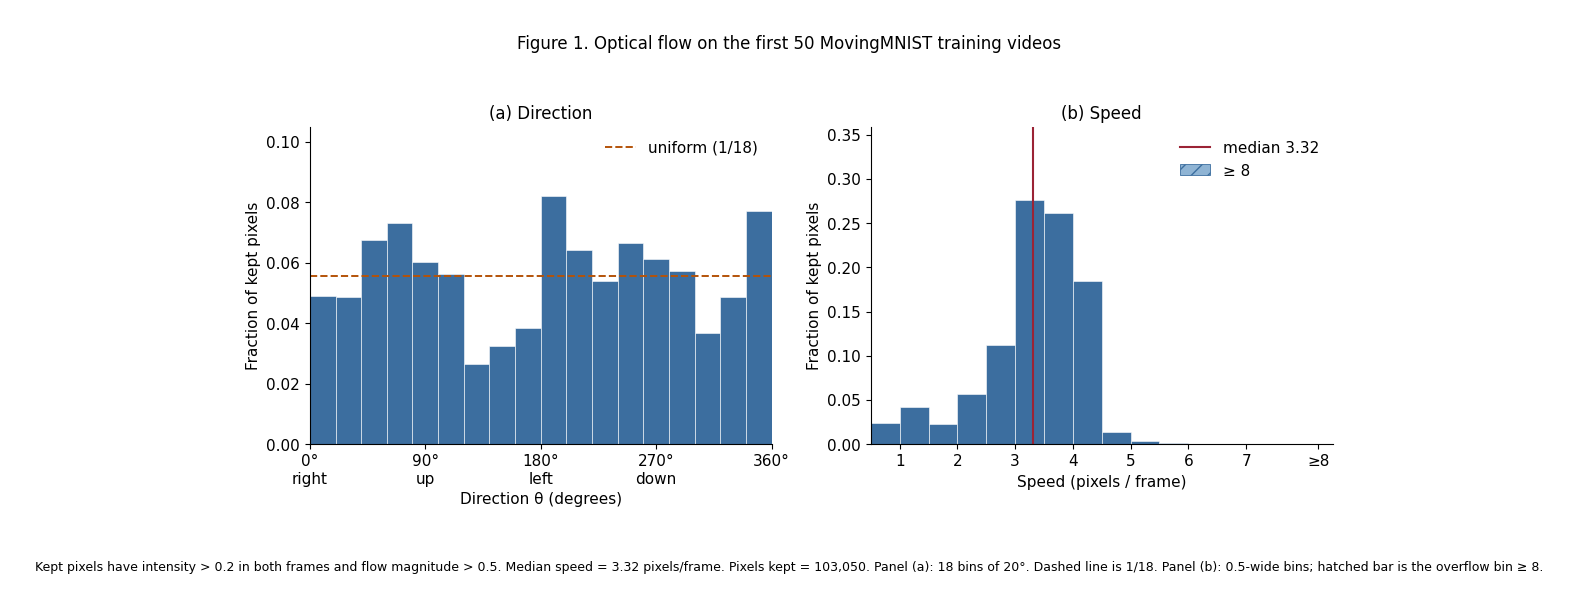
\includegraphics[width=\textwidth]{figure1.png}
\caption{Figure 1. Farneback optical flow on the first 50 training videos, 950 frame pairs. Pixels kept have intensity above 0.2 in both frames and flow magnitude above 0.5. Median speed is 3.32 pixels/frame. Pixels kept: 103{,}050. Panel (a): 18 bins of \(20^{\circ}\), dashed line at \(1/18\). Panel (b): 0.5-wide bins; the hatched bar is the overflow at or above 8.}
\end{figure}

\textbf{Q2.1.} Mirrored and rotated trajectories are only partly familiar. Every \(20^{\circ}\) bin in Figure~1(a) is occupied, so neither transform introduces a compass direction that is absent. The histogram is not uniform. The tallest bin is \([180^{\circ},200^{\circ})\) at fraction 0.0820, then \([340^{\circ},360^{\circ})\) at 0.0772 and \([60^{\circ},80^{\circ})\) at 0.0731. The shortest is \([120^{\circ},140^{\circ})\) at 0.0263. A horizontal mirror sends \(\theta\) to \(180^{\circ}-\theta\) and moves 13.2\% of the kept pixels into a different bin. A \(90^{\circ}\) anticlockwise rotation moves 20.0\%. Directions that occur are not the same as the proportions the training sample shows.

A typical speed is the median, 3.32 pixels/frame. The interquartile range is 3.00 to 3.89, and 0.835 of kept pixels lie between 2.5 and 4.5. Twice the median is 6.64 pixels/frame and three times it is 9.95. Both sit outside the body of Figure~1(b). The 99th percentile at \(1\times\) is 4.67, and only 0.00465 of kept pixels exceed 5. Overlap can scatter a minority of Farneback vectors. It is too small to move the median off 3.32 or to bring 6.64 or 9.95 into the main mass, and too small to flatten the direction histogram.

\textbf{Q2.2.} Mirror changes the glyph and the direction statistics. Speed is unchanged, because flipping the sign of \(dx\) does not change the magnitude. Rotation changes the glyph further and adds \(90^{\circ}\) to every flow angle. Speed is again unchanged. Speed-up leaves each displayed glyph as an original frame and multiplies the step between successive observed frames by two or three. The three edits separate appearance, direction, and speed.

\subsection{Model A, Table 2, Figure 2, Q2.3--Q2.4}

Model A folds each frame with \texttt{pixel\_unshuffle(4)}, runs two ConvLSTM layers with 64 hidden channels and \(3\times 3\) kernels, maps 64 channels to 16 with a \(1\times 1\) convolution, and returns a frame with \texttt{pixel\_shuffle(4)} and a sigmoid. One convolution produces the four gates. There are no peepholes. The rollout is nine steps. Steps 1--5 read the real frames. Steps 6--9 read the network's own previous prediction, and the gradient is not stopped. Outputs of steps 5--9 are the forecast. The parameter count is 480{,}784: layer 1 has 184{,}576, layer 2 has 295{,}168, and the head has 1{,}040.

Training used Adam at \(10^{-3}\), batch 32, 30 epochs, and the final-epoch weights. One epoch is one shuffled pass over the 8{,}000 training videos with one random legal window. On the Tesla T4 a training epoch took 11.3 seconds. Inference on the 1{,}000 original test clips took 0.461 seconds.

\begin{table}[H]
\centering
\caption{Table 2. Test error at \(1\times\), \(t=1\). Model A is the mean (seed 0, seed 1).}
\begin{tabular}{lccc}
\toprule
 & Model A & Blank & Copy-last \\
\midrule
MSE\(_1\) & 0.0169 (0.0174, 0.0164) & 0.0426 & 0.0492 \\
MSE\(_2\) & 0.0203 (0.0209, 0.0198) & 0.0426 & 0.0604 \\
MSE\(_3\) & 0.0226 (0.0231, 0.0221) & 0.0426 & 0.0669 \\
MSE\(_4\) & 0.0244 (0.0248, 0.0240) & 0.0425 & 0.0708 \\
MSE\(_5\) & 0.0261 (0.0264, 0.0257) & 0.0425 & 0.0732 \\
\(E(5)\) & 0.0221 (0.0225, 0.0216) & 0.0426 & 0.0641 \\
Parameters & 480{,}784 & 0 & 0 \\
\bottomrule
\end{tabular}
\end{table}

\begin{figure}[H]
\centering
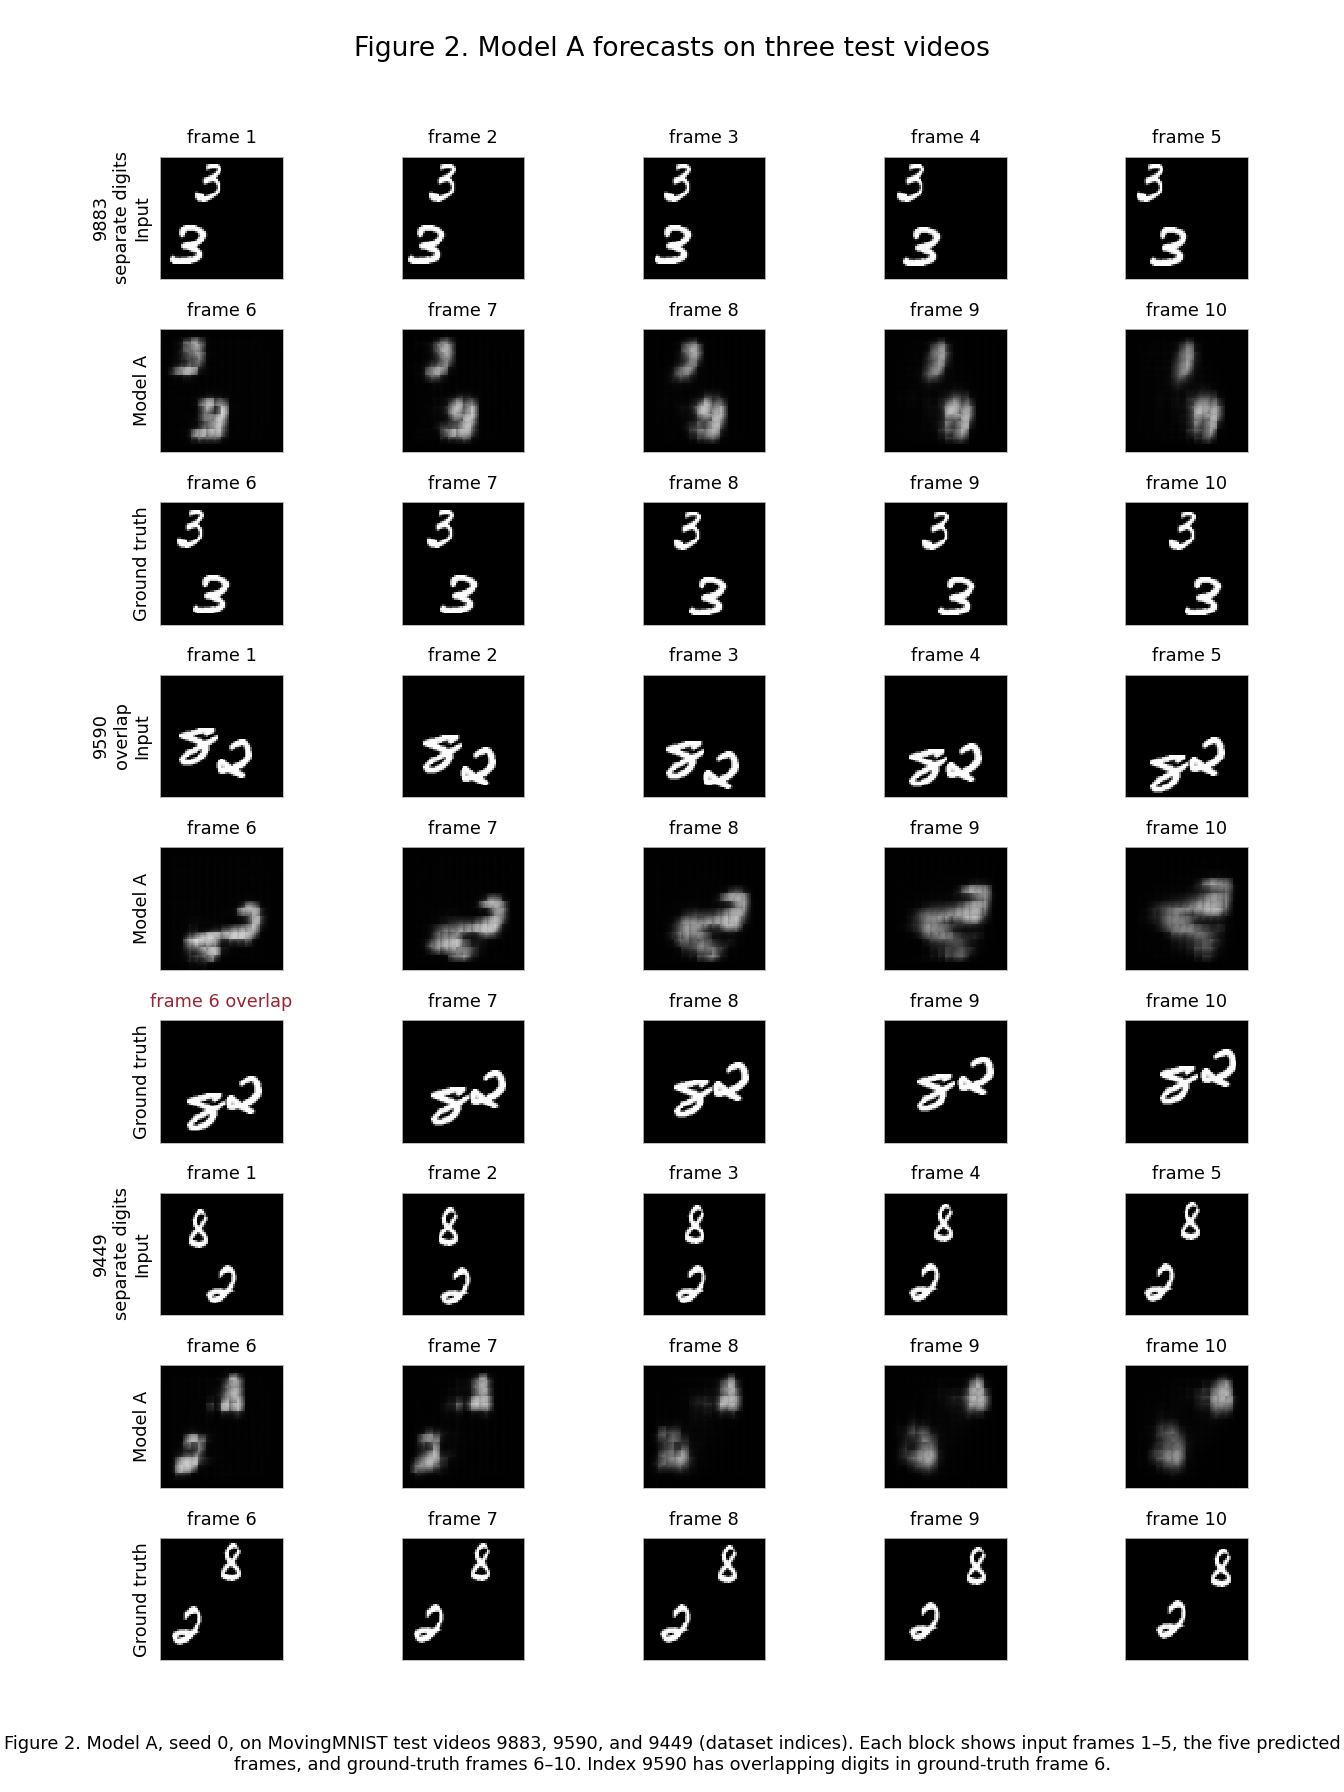
\includegraphics[width=\textwidth]{figure2.png}
\caption{Figure 2. Model A, seed 0, on test videos 9883, 9590, and 9449. Each block shows input frames 1--5, the five predicted frames, and ground-truth frames 6--10. Index 9590 has overlapping digits in ground-truth frame 6.}
\end{figure}

\textbf{Q2.3.} Model A's one-step reach is 8 original pixels. \texttt{pixel\_unshuffle(4)} leaves a \(16\times 16\) grid whose neighbouring cells are 4 original pixels apart, centre to centre. The fold, the \(1\times 1\) head, and \texttt{pixel\_shuffle} do not move information to another cell. Each \(3\times 3\) kernel moves one folded cell. Inside one step the new input passes through layer 1 and then through layer 2, which reads layer 1's new hidden state. That is two cells, \(2\times 4 = 8\) original pixels. The previous hidden state of layer 1 travels the same two kernels. The previous hidden state of layer 2 travels only one, which is 4 original pixels. The longest path is \(u_{\tau}\rightarrow\) layer-1 \(3\times 3\rightarrow h^{(1)}_{\tau}\rightarrow\) layer-2 \(3\times 3\rightarrow\hat x_{\tau+1}\).

\textbf{Q2.4.} At \(1\times\), Model A's \(E(5)\) of 0.0221 is below Blank (0.0426) and below Copy-last (0.0641) at every horizon. The seed-mean error grows from 0.0169 at horizon 1 to 0.0261 at horizon 5, and the steps between horizons shrink. Horizon 5 is still below Blank. Copy-last is worse than Blank because repeating frame 5 leaves ink where the digit has left and misses where it has gone. On videos 9883 and 9449 the two digits stay apart and the forecast is a soft mark near each digit that spreads by frame 10. On 9590 the digits cross. The seed-0 forecast draws one soft shape for the pair and is still one smear at frames 9 and 10, where the truth has separated.

\subsection{Q2.5}

This answer was committed as \texttt{10cb5f4} at 14:35 on 27 October 2026, before the mirror, rotation, and speed tests. It is unchanged.

Model A will not pass the mirror test. Its one-step reach is 8 original pixels, which is a statement about how far a \(3\times 3\) convolution can move information, not about reflection. The filters are ordinary convolutions, with no mirrored copy of the weights. Figure~1(a) is not symmetric under a horizontal flip: reflecting the measured flow sends \(\theta\) to \(180^{\circ}-\theta\) and moves 13.2\% of the 103{,}050 kept pixels into a different \(20^{\circ}\) bin. A mirrored digit is also a different glyph. Both the direction balance and the appearance sit outside the \(1\times\) training sample, so \(f(M(X))\) should disagree with \(M(f(X))\) and with \(M(Y)\).

Model A will not pass the rotation test, and rotation should be worse than mirroring. A \(90^{\circ}\) anticlockwise turn changes the glyph further than a left-right flip, and on these same pixels it reassigns 20.0\% of the kept flow into a different bin. Nothing in the two-layer ConvLSTM ties a filter to its quarter-turn.

It should break at \(3\times\), and \(2\times\) should already be strained for the faster digits. The median consecutive-frame speed is 3.32 pixels per frame, inside the 8-pixel reach. Twice that median is 6.64, still under 8 but close. The 99th percentile at \(1\times\) is 4.67, which becomes about 9.3 at \(2\times\) and is already past the reach. Three times the median is 9.95, beyond 8.

\subsection{Tables 3--4 and Figures 3--5}

\begin{table}[H]
\centering
\caption{Table 3. Consistency and transformed error at \(1\times\), \(t=1\). Blank and Copy-last have \(C_M=C_R=0\).}
\small
\begin{tabular}{lccc}
\toprule
 & Model A & Blank & Copy-last \\
\midrule
\(E(5)\) & 0.0221 (0.0225, 0.0216) & 0.0426 & 0.0641 \\
\(C_M\) & 0.00183 (0.00168, 0.00198) & 0 & 0 \\
\(E_M\) & 0.0227 (0.0232, 0.0223) & 0.0426 & 0.0641 \\
\(C_R\) & 0.00308 (0.00315, 0.00302) & 0 & 0 \\
\(E_R\) & 0.0238 (0.0242, 0.0234) & 0.0426 & 0.0641 \\
\bottomrule
\end{tabular}
\end{table}

\begin{figure}[H]
\centering
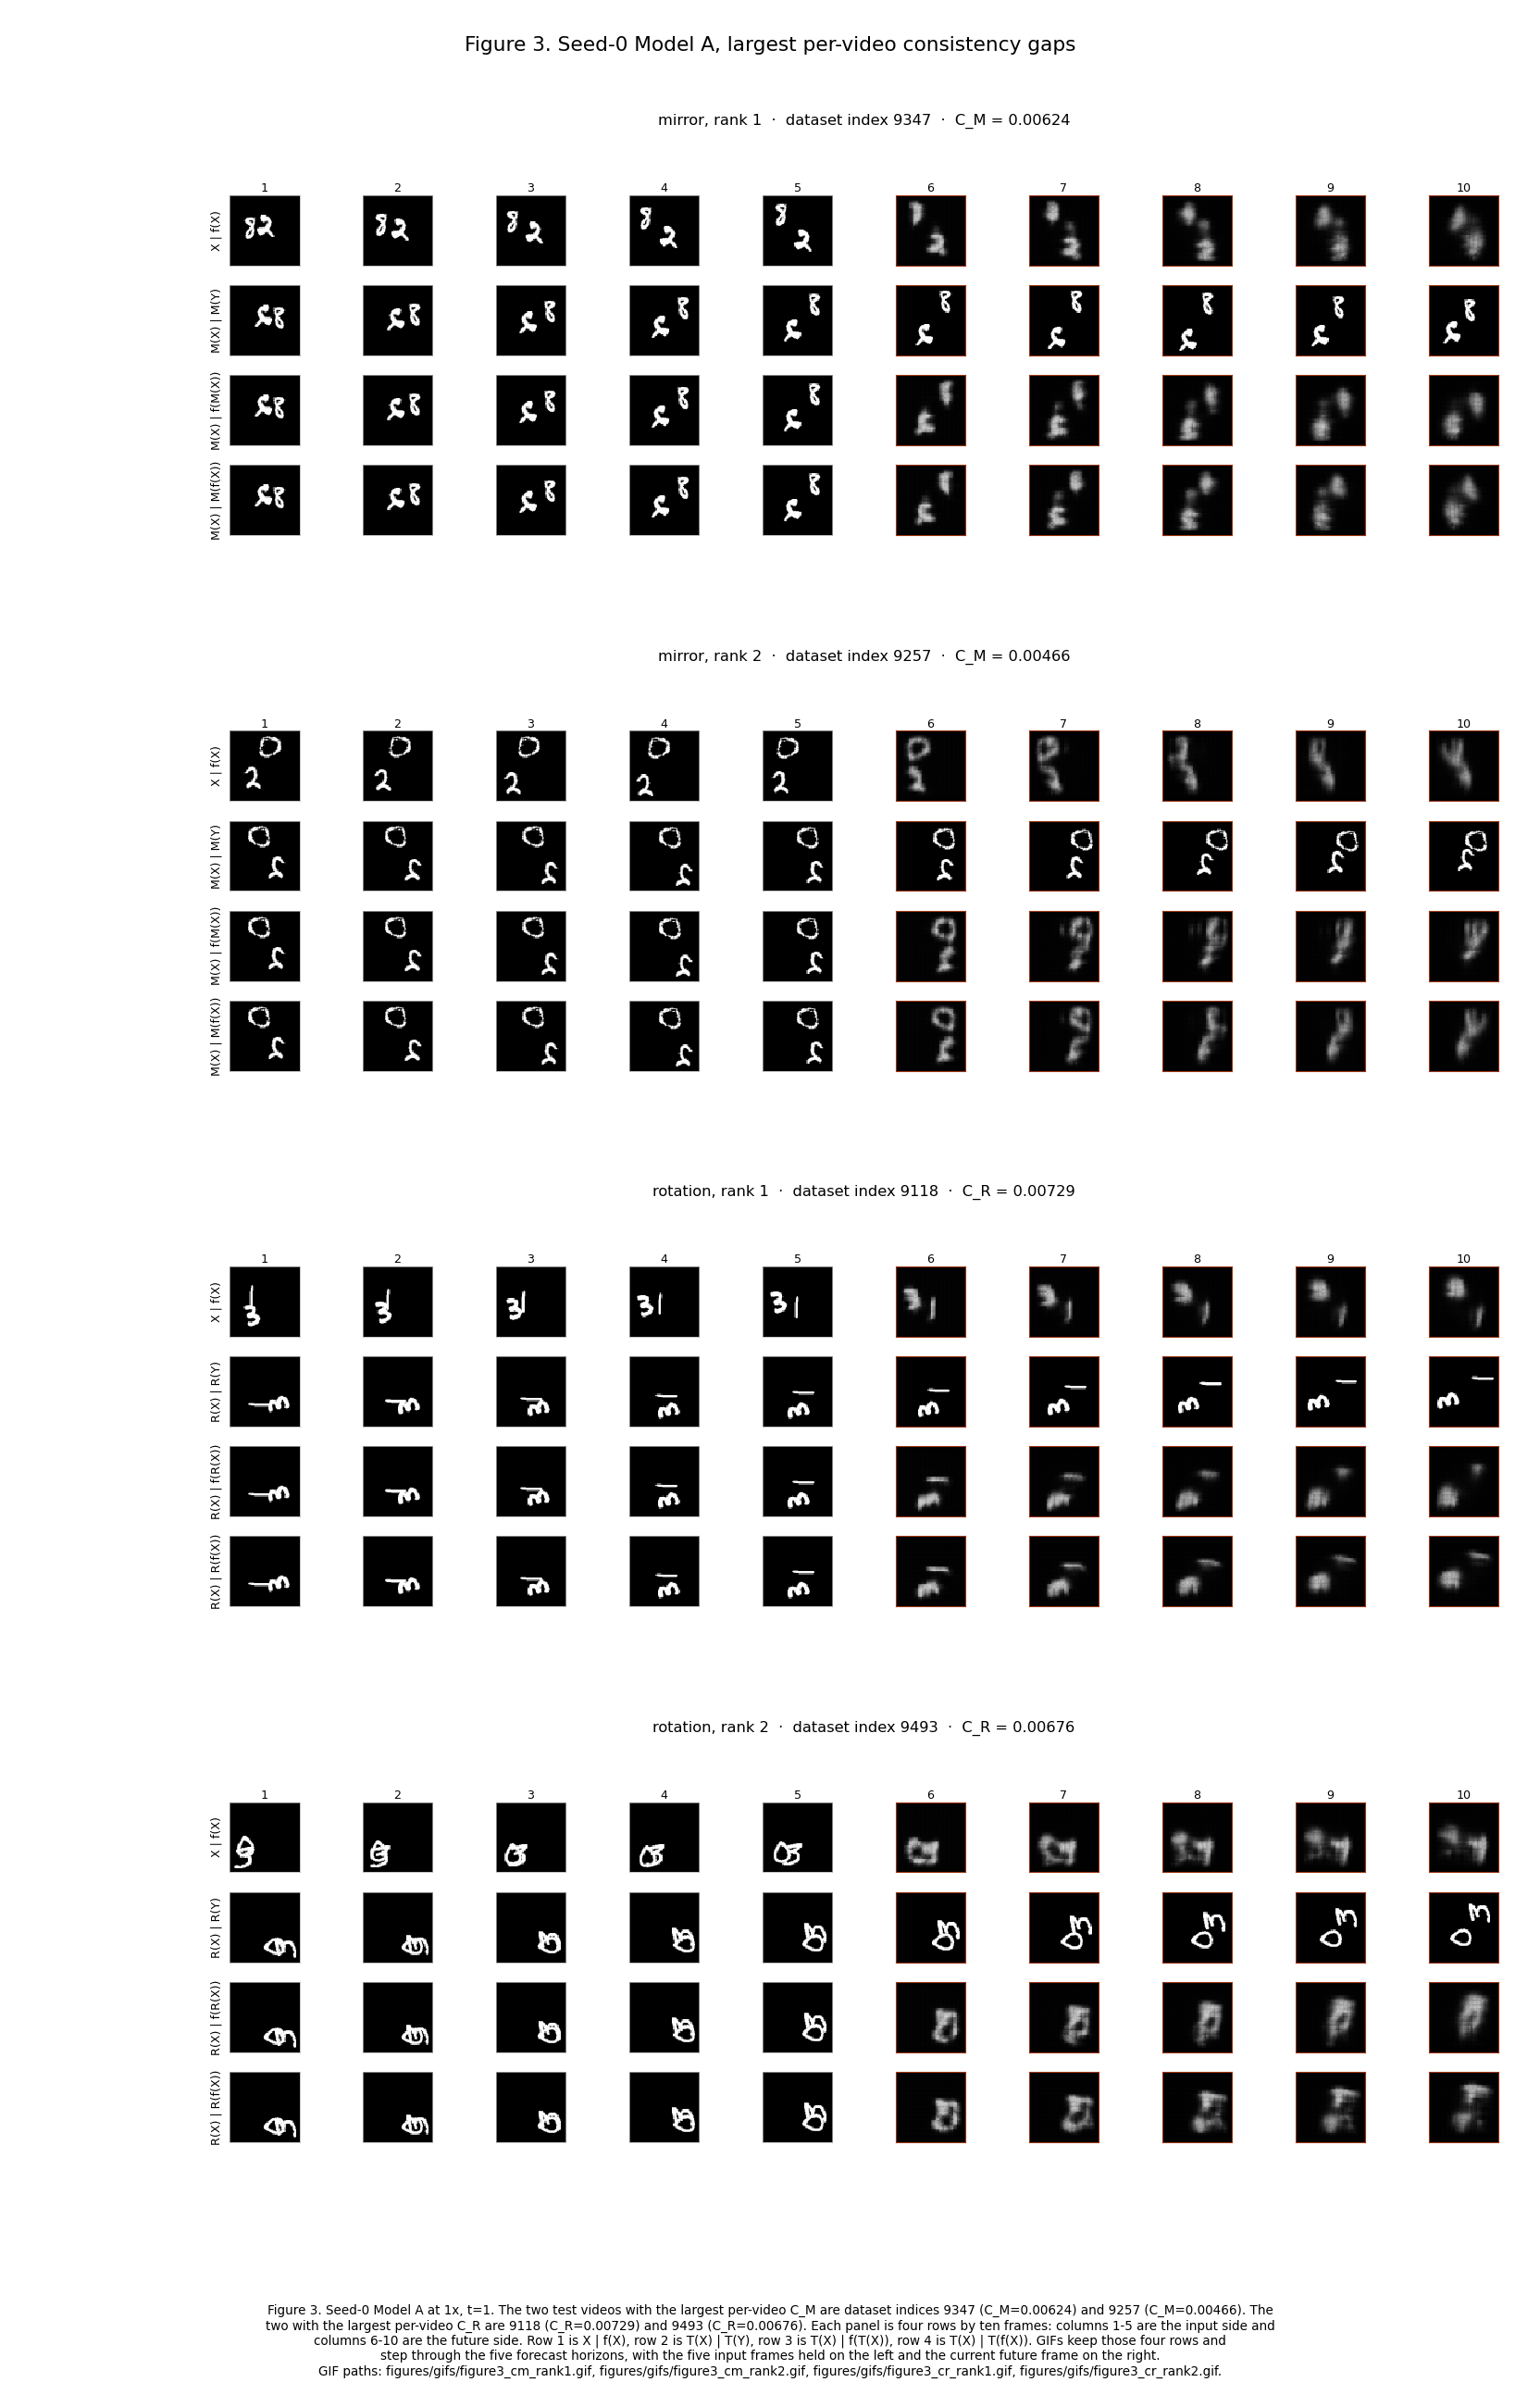
\includegraphics[width=\textwidth,height=0.78\textheight,keepaspectratio]{figure3.png}
\caption{Figure 3. Seed-0 Model A. Mirror ranks are test videos 9347 (\(C_M=0.00624\)) and 9257 (\(C_M=0.00466\)). Rotation ranks are 9118 (\(C_R=0.00729\)) and 9493 (\(C_R=0.00676\)). Each panel has four rows: \(X\mid f(X)\); \(T(X)\mid T(Y)\); \(T(X)\mid f(T(X))\); \(T(X)\mid T(f(X))\). GIFs: \texttt{figures/gifs/figure3\_cm\_rank1.gif}, \texttt{figures/gifs/figure3\_cm\_rank2.gif}, \texttt{figures/gifs/figure3\_cr\_rank1.gif}, \texttt{figures/gifs/figure3\_cr\_rank2.gif}.}
\end{figure}

\begin{figure}[H]
\centering
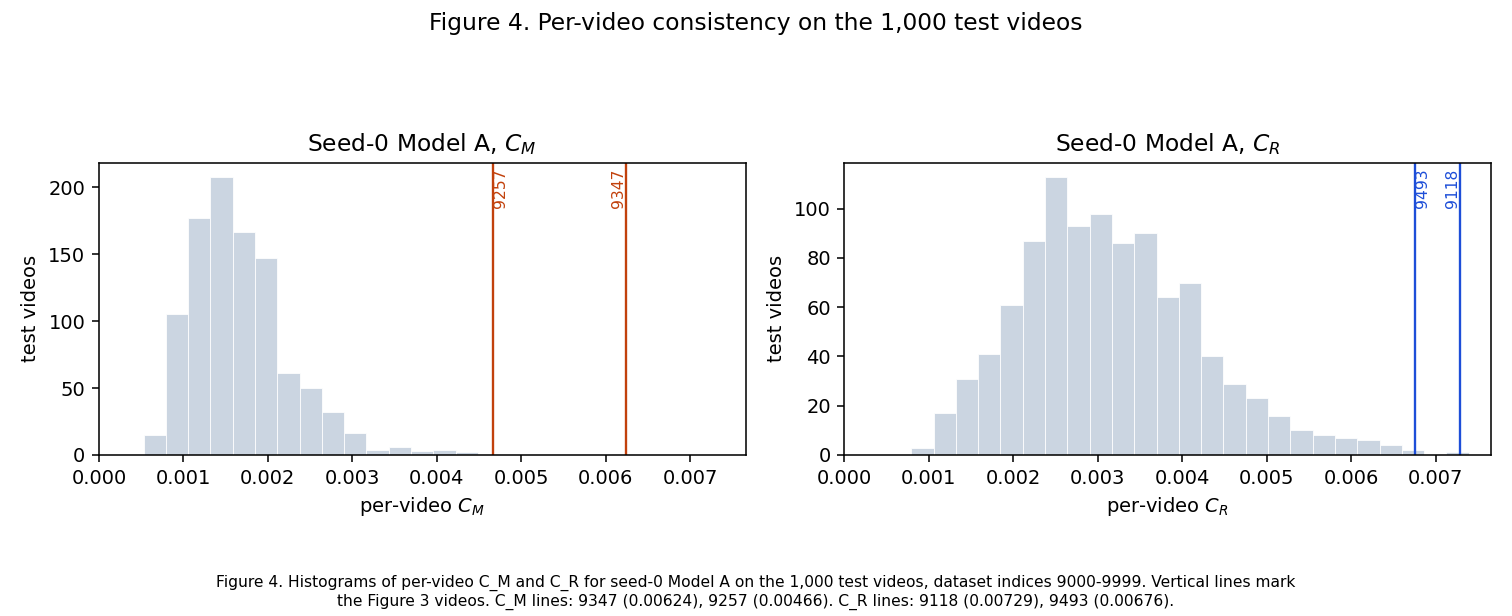
\includegraphics[width=0.92\textwidth]{figure4.png}
\caption{Figure 4. Per-video \(C_M\) and \(C_R\) of seed-0 Model A on the 1{,}000 test videos. The Figure~3 videos are marked.}
\end{figure}

\begin{table}[H]
\centering
\caption{Table 4. Speed comparison at \(t=1\). \(E(5)\) is not reported at \(3\times\).}
\begin{tabular}{lcc}
\toprule
 & Model A & Copy-last \\
\midrule
\(E(2)\), \(1\times\) & 0.0186 (0.0191, 0.0181) & 0.0548 \\
\(E(2)\), \(2\times\) & 0.0448 (0.0449, 0.0448) & 0.0661 \\
\(E(2)\), \(3\times\) & 0.0520 (0.0528, 0.0511) & 0.0703 \\
\(E(5)\), \(1\times\) & 0.0221 (0.0225, 0.0216) & 0.0641 \\
\(E(5)\), \(2\times\) & 0.0490 (0.0486, 0.0493) & 0.0719 \\
\bottomrule
\end{tabular}
\end{table}

\begin{figure}[H]
\centering
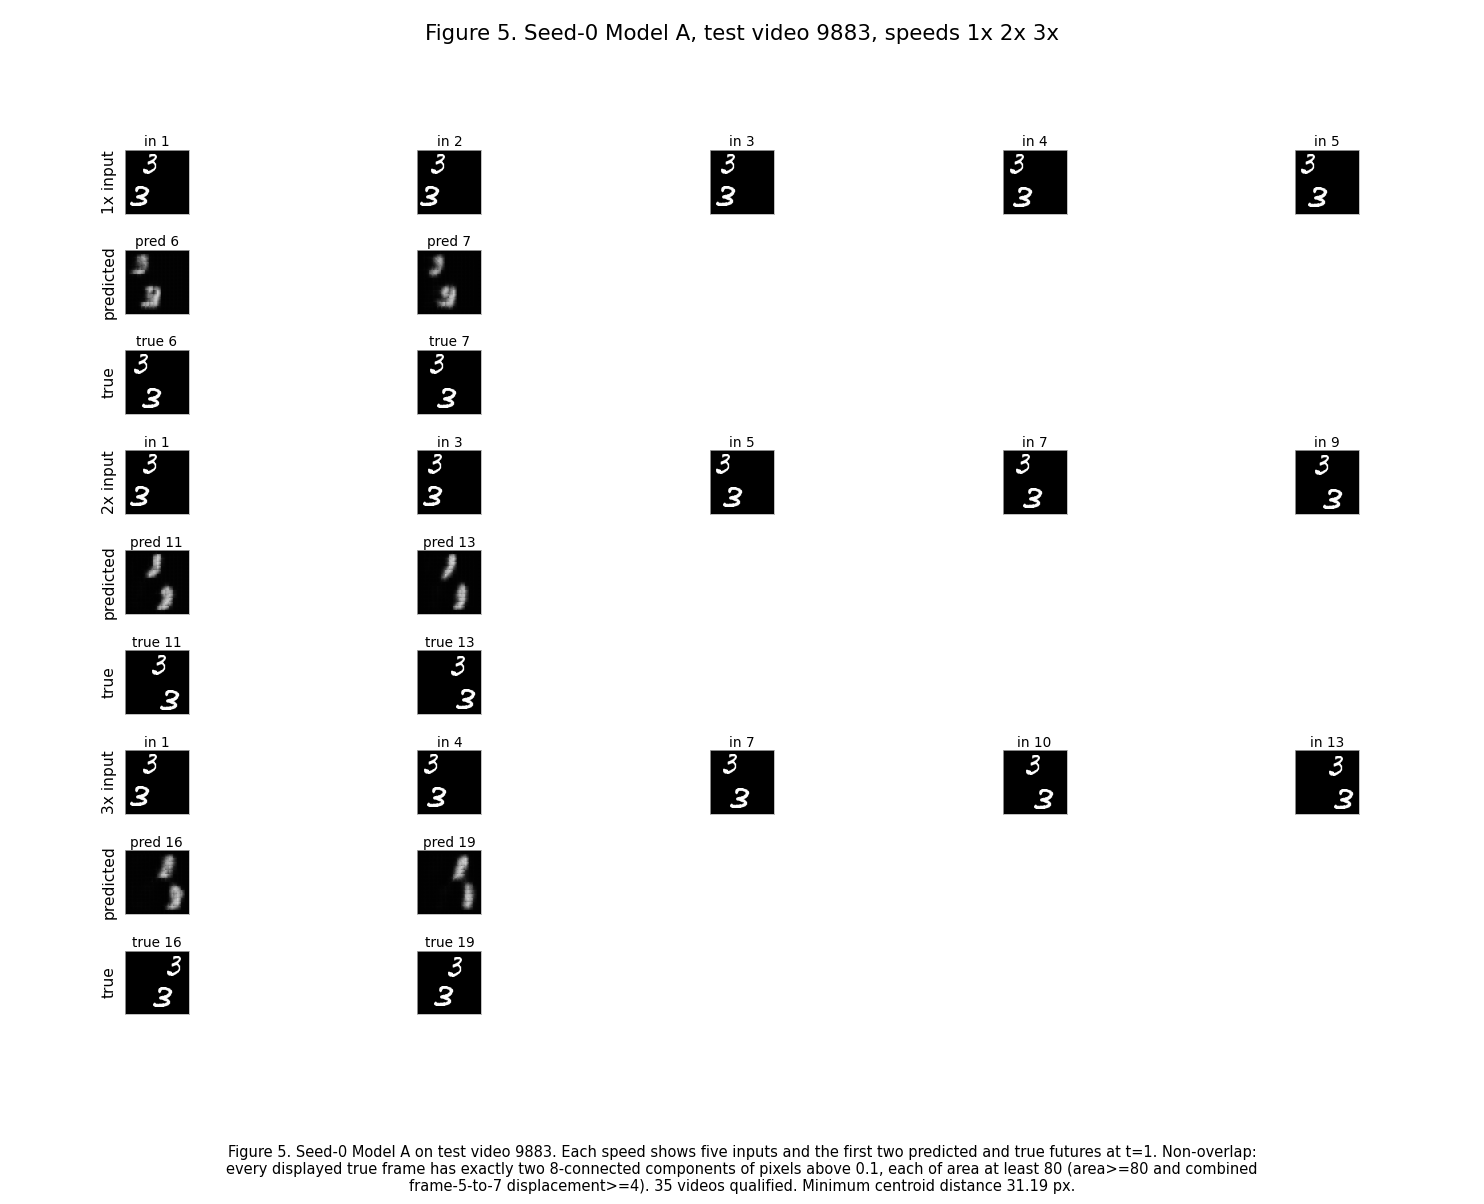
\includegraphics[width=\textwidth]{figure5.png}
\caption{Figure 5. Seed-0 Model A on test video 9883. Five inputs and the first two predicted and true futures at \(1\times\), \(2\times\), and \(3\times\). The displayed true frames do not contain overlapping digits.}
\end{figure}

\textbf{Q2.6.} Blank and Copy-last have \(C_M=C_R=0\) because both maps commute with mirror and rotation: an all-zero frame stays zero, and mirroring or rotating a repeated last frame is the same as repeating the transformed last frame. A consistency gap of zero does not mean the forecast is right. Blank's \(E_M\) and \(E_R\) equal its \(E(5)\) of 0.0426, and Copy-last's equal 0.0641. \(C_T\) has to be read next to \(E_T\).

\textbf{Q2.7.} The video is Figure~3, mirror rank 1, dataset 9347, seed 0. Row 3, \(f(M(X))\), still has two digits at horizon 5, with the second digit too far down and not far enough left. Row 4, \(M(f(X))\), is one blob, because the original forecast has already become one component and a mirror cannot split a component. The per-video \(C_M\) is 0.00624. The model accounts for the mirrored clip as two marks and for the mirrored original forecast as one.

\textbf{Q2.8.} Rotation is harder than mirroring for Model A. Mean \(C_R\) is 0.00308 against \(C_M\) of 0.00183, and mean \(E_R\) is 0.0238 against \(E_M\) of 0.0227. Q2.1 and Q2.2 say both transforms change the glyph and the direction histogram, and rotation moves more of the flow (20.0\% against 13.2\%) and changes the glyph further. The speed is the same under both, so the extra error is appearance and direction, not a faster step.

\textbf{Q2.9.} Model A's predictions fall apart at \(2\times\), and \(3\times\) is worse. \(E(2)\) rises from 0.0186 at \(1\times\) to 0.0448 at \(2\times\), which is already above Blank's 0.0426, and to 0.0520 at \(3\times\). The \(2\times\) median step of 6.64 is inside the 8-pixel reach, so the reach estimate missed that a step near the edge, and the fast tail past 8, is enough to break the forecast before the typical \(3\times\) step of 9.95. In Figure~5 the \(1\times\) forecast still follows the two digits. At \(2\times\) and \(3\times\) it becomes one soft blob that does not keep both trajectories.

\textbf{Q2.10.} These results do not separate ``fast motion was absent in training'' from ``the step is beyond the reach.'' Model A never saw \(2\times\) or \(3\times\), and its reach is 8. The experiment that separates them is Models C and D, which are not trained in this section. Model C keeps Model A's architecture and adds speed augmentation. Model D keeps that speed schedule and lengthens the reach. If C repairs \(2\times\) and still fails where the step exceeds 8 pixels, while D does better there, the remainder is reach. If C repairs both speeds, the failure was unfamiliar motion.

\subsection{Q2.11}

This answer was committed as \texttt{ede80b4} at 16:20 on 27 October 2026, before training B, C, and D. It is unchanged.

Model B should close the mirror and rotation gaps, the rotation gap most of all, because it trains on the group \(G\), and it should not fix the speed failure because it never sees \(2\times\) or \(3\times\). Model C should improve \(2\times\) if that error is unfamiliar motion inside the 8-pixel reach, and it should leave \(3\times\) broken, because a typical \(3\times\) step is 9.95 pixels and C still has Model A's reach. Model D, with reach 16 and the same speed schedule as C, is the one that should fix the \(3\times\) failure, and the part of the \(2\times\) failure that sits near the edge of 8 pixels.

\subsection{Models B, C, and D}

Model B is Model A trained at \(1\times\) with one uniform draw from the eight elements of \(G\) applied to the input and the target. Model C is Model A trained with \(k\) drawn from \(\{1,2,3\}\) and no symmetry augmentation. Model D is the same schedule as C, with dilation 2 and padding 2 on both \(3\times 3\) layers. Dilation does not add weights, so D also has 480{,}784 parameters, under the cap of 721{,}176. No attention is used.

\textbf{Q2.12.} Model D's one-step reach is 16 original pixels, against Model A's 8. A \(3\times 3\) kernel with dilation 2 reads offsets \(-2,0,+2\), so one layer moves 2 folded cells, which is 8 original pixels. The new input passes through both layers, and layer 2 reads layer 1's new hidden state, so the longest path is 4 folded cells, \(4\times 4 = 16\). The path is \(u_{\tau}\rightarrow\) layer-1 dilated \(3\times 3\rightarrow h^{(1)}_{\tau}\rightarrow\) layer-2 dilated \(3\times 3\rightarrow\hat x_{\tau+1}\). The \(1\times 1\) head and the shuffles add nothing. The previous state of layer 2 travels only one dilated kernel, which is 8 original pixels.

\begin{table}[H]
\centering
\caption{Table 5. Test metrics for A--D. Consistency is at \(1\times\). \(E(2)\) at \(3\times\) uses the first two horizons only. Training and inference times are seconds on a Tesla T4.}
\scriptsize
\resizebox{\textwidth}{!}{%
\begin{tabular}{lcccc}
\toprule
 & A & B & C & D \\
\midrule
\(E(5)\), \(1\times\) & 0.0221 (0.0225, 0.0216) & 0.0223 (0.0226, 0.0221) & 0.0267 (0.0268, 0.0267) & 0.0287 (0.0283, 0.0290) \\
\(C_M\) & 0.00183 (0.00168, 0.00198) & 0.00106 (0.00108, 0.00105) & \(9.30\times10^{-4}\) & \(9.81\times10^{-4}\) \\
\(E_M\) & 0.0227 (0.0232, 0.0223) & 0.0224 (0.0227, 0.0221) & 0.0269 (0.0270, 0.0269) & 0.0289 (0.0286, 0.0292) \\
\(C_R\) & 0.00308 (0.00315, 0.00302) & 0.00132 (0.00126, 0.00139) & 0.00205 (0.00188, 0.00222) & 0.00181 (0.00166, 0.00197) \\
\(E_R\) & 0.0238 (0.0242, 0.0234) & 0.0223 (0.0226, 0.0219) & 0.0279 (0.0279, 0.0278) & 0.0296 (0.0292, 0.0299) \\
\(E(2)\), \(1\times\) & 0.0186 (0.0191, 0.0181) & 0.0186 (0.0187, 0.0184) & 0.0230 (0.0230, 0.0230) & 0.0263 (0.0261, 0.0266) \\
\(E(2)\), \(2\times\) & 0.0448 (0.0449, 0.0448) & 0.0446 (0.0444, 0.0448) & 0.0288 (0.0288, 0.0289) & 0.0293 (0.0289, 0.0297) \\
\(E(2)\), \(3\times\) & 0.0520 (0.0528, 0.0511) & 0.0506 (0.0496, 0.0515) & 0.0335 (0.0336, 0.0334) & 0.0316 (0.0311, 0.0321) \\
Parameters & 480{,}784 & 480{,}784 & 480{,}784 & 480{,}784 \\
s/epoch & 11.3 & 11.6 & 12.4 & 19.9 \\
Inference (s) & 0.461 & 0.464 & 0.453 & 0.720 \\
\bottomrule
\end{tabular}}
\end{table}

Model C's seed pair for \(C_M\) is \(8.82\times10^{-4}\) and \(9.77\times10^{-4}\). Model D's is \(9.90\times10^{-4}\) and \(9.71\times10^{-4}\).

\textbf{Q2.13.} The mirror gap and the rotation gap of Model A at \(1\times\) are appearance. Model B, same architecture and no new speeds, cuts \(C_M\) from 0.00183 to 0.00106 and \(C_R\) from 0.00308 to 0.00132, and its transformed errors sit on its own \(E(5)\) of 0.0223. Its \(2\times\) and \(3\times\) errors stay with Model A. Model C, which never trains on the mirror or the rotation, does not restore \(E_M\) or \(E_R\).

The \(2\times\) failure is unfamiliar motion. Model C has the same 8-pixel reach and has seen \(2\times\) windows. Its \(E(2)\) at \(2\times\) is 0.0288, against Model A's 0.0448 and Model B's 0.0446. Model D, with the longer reach and the same speed schedule, is level with C at \(2\times\) (0.0293). A typical \(2\times\) step of 6.64 pixels is inside the 8-pixel path.

The \(3\times\) failure is unfamiliar motion and then reach. Model C's \(E(2)\) at \(3\times\) is 0.0335, below Model A's 0.0520 and Model B's 0.0506, so seeing the fast step helps while the reach is still 8. Model D's \(E(2)\) at \(3\times\) is 0.0316, below both seeds of Model C. The two models share the speed schedule and differ by the dilation. A typical \(3\times\) step is 9.95 pixels, past 8 and inside 16. More \(3\times\) examples cannot add the extra folded cells. The gradient only changes weights on paths the forward pass already has, and Model C's paths stop at 8 original pixels.

\textbf{Q2.14.} Model B does not cost accuracy on the original \(1\times\) clips. Its \(E(5)\) is 0.0223 against Model A's 0.0221. The symmetry training was worth it: the mirror and rotation gaps shrink and the transformed errors stay level with \(E(5)\). Model C's \(E(5)\) at \(1\times\) rises to 0.0267. The same training cuts \(E(2)\) at \(2\times\) by 0.0160 and at \(3\times\) by 0.0185, both larger than the 0.00467 rise on the original clips, so the speed change was worth it for the fast clips and is a real loss on the ordinary ones. Model D's \(E(5)\) at \(1\times\) is 0.0287, the highest of the four. The dilation was worth it at \(3\times\), where D is the lowest, and it was not worth it on the original clips, whose median step of 3.32 already fits inside Model A's reach. Against C, the \(1\times\) cost of about 0.00193 is the same size as the \(3\times\) gain of about 0.00185.

\subsection{The final model}

Table 5 supports D+B. Model B cut the rotation gap without moving \(E(5)\), and Model D's rotation gap (0.00181) was still larger than its mirror gap. D+B is Model D trained with both the speed draw and one shared group element on each window. Its \(E(5)\) is 0.0285 (0.0287, 0.0282), slightly under D. Its gaps are \(C_M=7.53\times10^{-4}\) and \(C_R=9.89\times10^{-4}\), with \(E_M=E_R=0.0285\). Its \(E(2)\) is 0.0261, 0.0290, and 0.0313 at \(1\times\), \(2\times\), and \(3\times\). The speed gains survive. The final model is that network wrapped as
\[
\bar f(X)=\frac{1}{8}\sum_{g\in G} g^{-1}\big(f(g(X))\big).
\]
For any \(h\in G\), right multiplication by \(h\) permutes \(G\) and \(h\) factors out of the average, so \(\bar f(h(X))=h(\bar f(X))\). Since \(M\) and \(R\) are in \(G\), \(C_M=C_R=0\) exactly. The measured gaps are the floating-point residual.

\begin{table}[H]
\centering
\caption{Table 6. Symmetrised forecasters. Training time is the underlying model's seconds per epoch. Inference includes all eight transforms. \(C_M\) and \(C_R\) are scientific notation.}
\scriptsize
\begin{tabular}{lccc}
\toprule
 & Sym.\ B & Sym.\ D & Sym.\ D+B (final) \\
\midrule
\(E(5)\), \(1\times\) & 0.0218 & 0.0285 & 0.0281 (0.0284, 0.0279) \\
\(C_M\) & \(8.43\times10^{-17}\) & \(5.47\times10^{-17}\) & \(5.65\times10^{-17}\) \\
\(E_M\) & 0.0218 & 0.0285 & 0.0281 \\
\(C_R\) & \(6.76\times10^{-17}\) & \(4.26\times10^{-17}\) & \(4.48\times10^{-17}\) \\
\(E_R\) & 0.0218 & 0.0285 & 0.0281 \\
\(E(2)\), \(1\times\) & 0.0181 & 0.0263 & 0.0259 (0.0261, 0.0257) \\
\(E(2)\), \(2\times\) & 0.0438 & 0.0291 & 0.0286 (0.0288, 0.0285) \\
\(E(2)\), \(3\times\) & 0.0495 & 0.0314 & 0.0309 (0.0311, 0.0306) \\
Parameters & 480{,}784 & 480{,}784 & 480{,}784 \\
s/epoch & 11.6 & 19.9 & 20.7 \\
Inference (s) & 3.81 & 5.24 & 4.95 \\
\bottomrule
\end{tabular}
\end{table}

\begin{figure}[H]
\centering
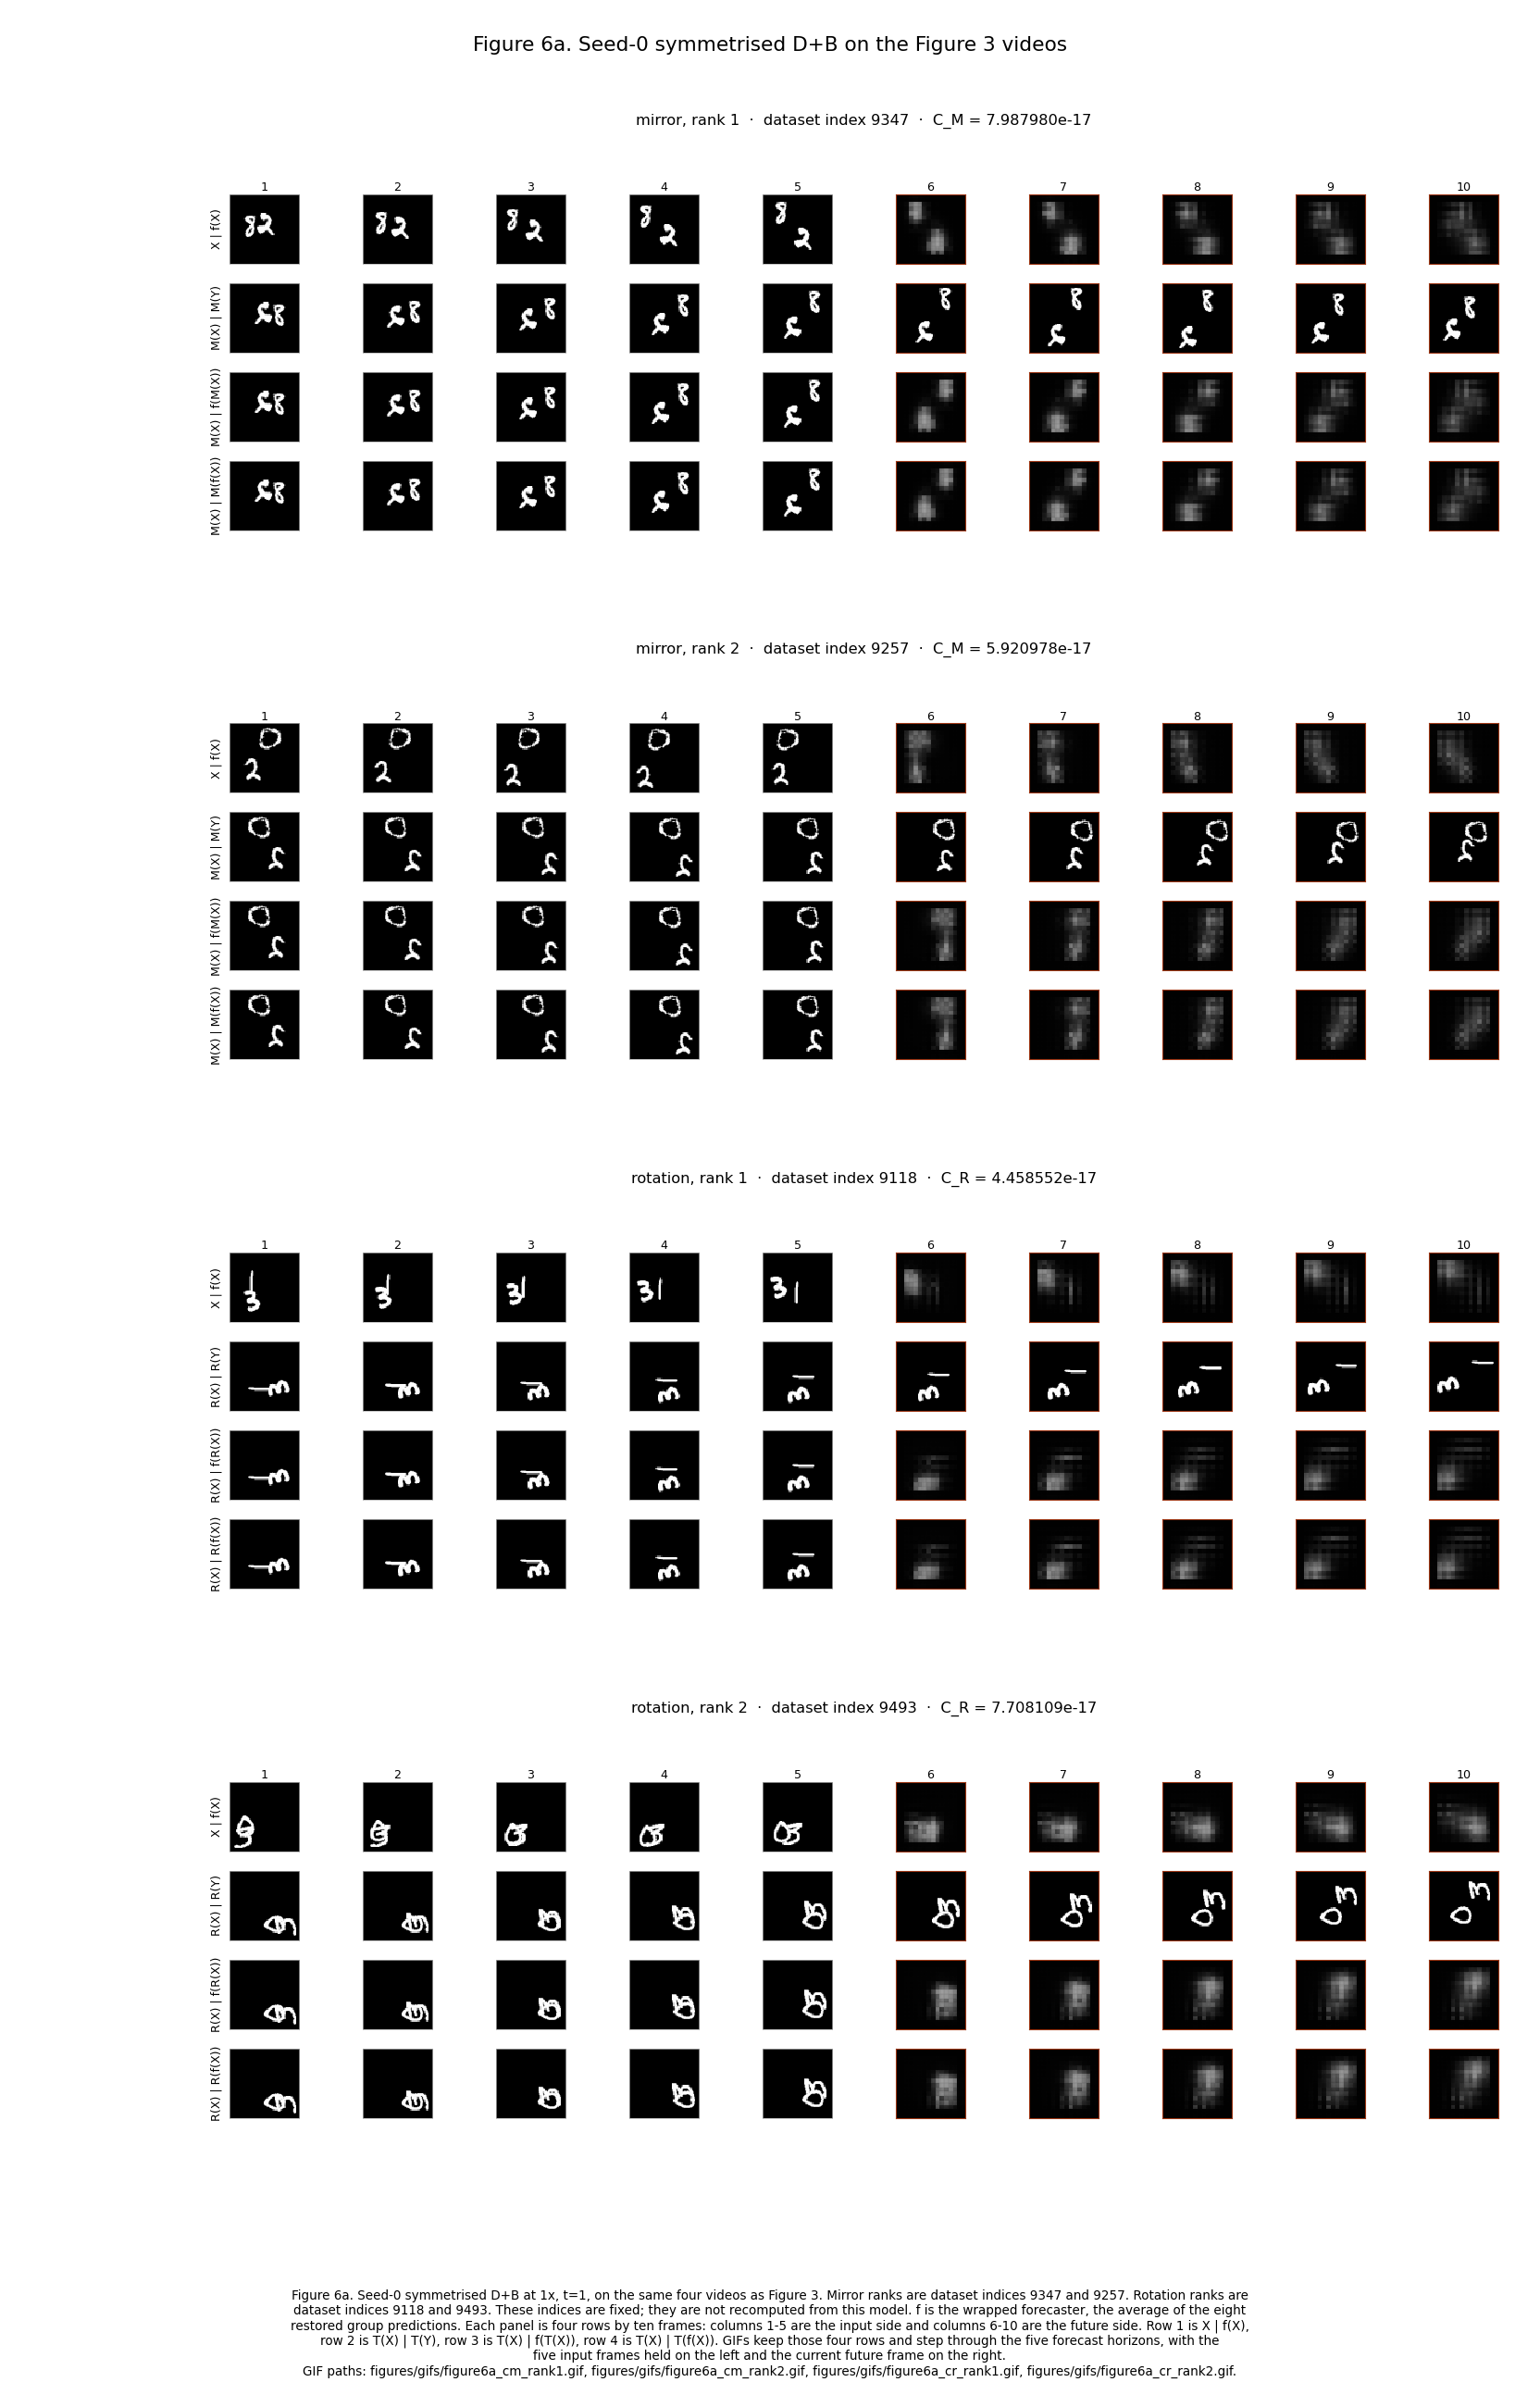
\includegraphics[width=\textwidth,height=0.78\textheight,keepaspectratio]{figure6a.png}
\caption{Figure 6(a). Symmetrised D+B, seed 0, on the Figure~3 videos: mirror 9347 and 9257, rotation 9118 and 9493. GIFs: \texttt{figures/gifs/figure6a\_cm\_rank1.gif}, \texttt{figures/gifs/figure6a\_cm\_rank2.gif}, \texttt{figures/gifs/figure6a\_cr\_rank1.gif}, \texttt{figures/gifs/figure6a\_cr\_rank2.gif}.}
\end{figure}

\begin{figure}[H]
\centering
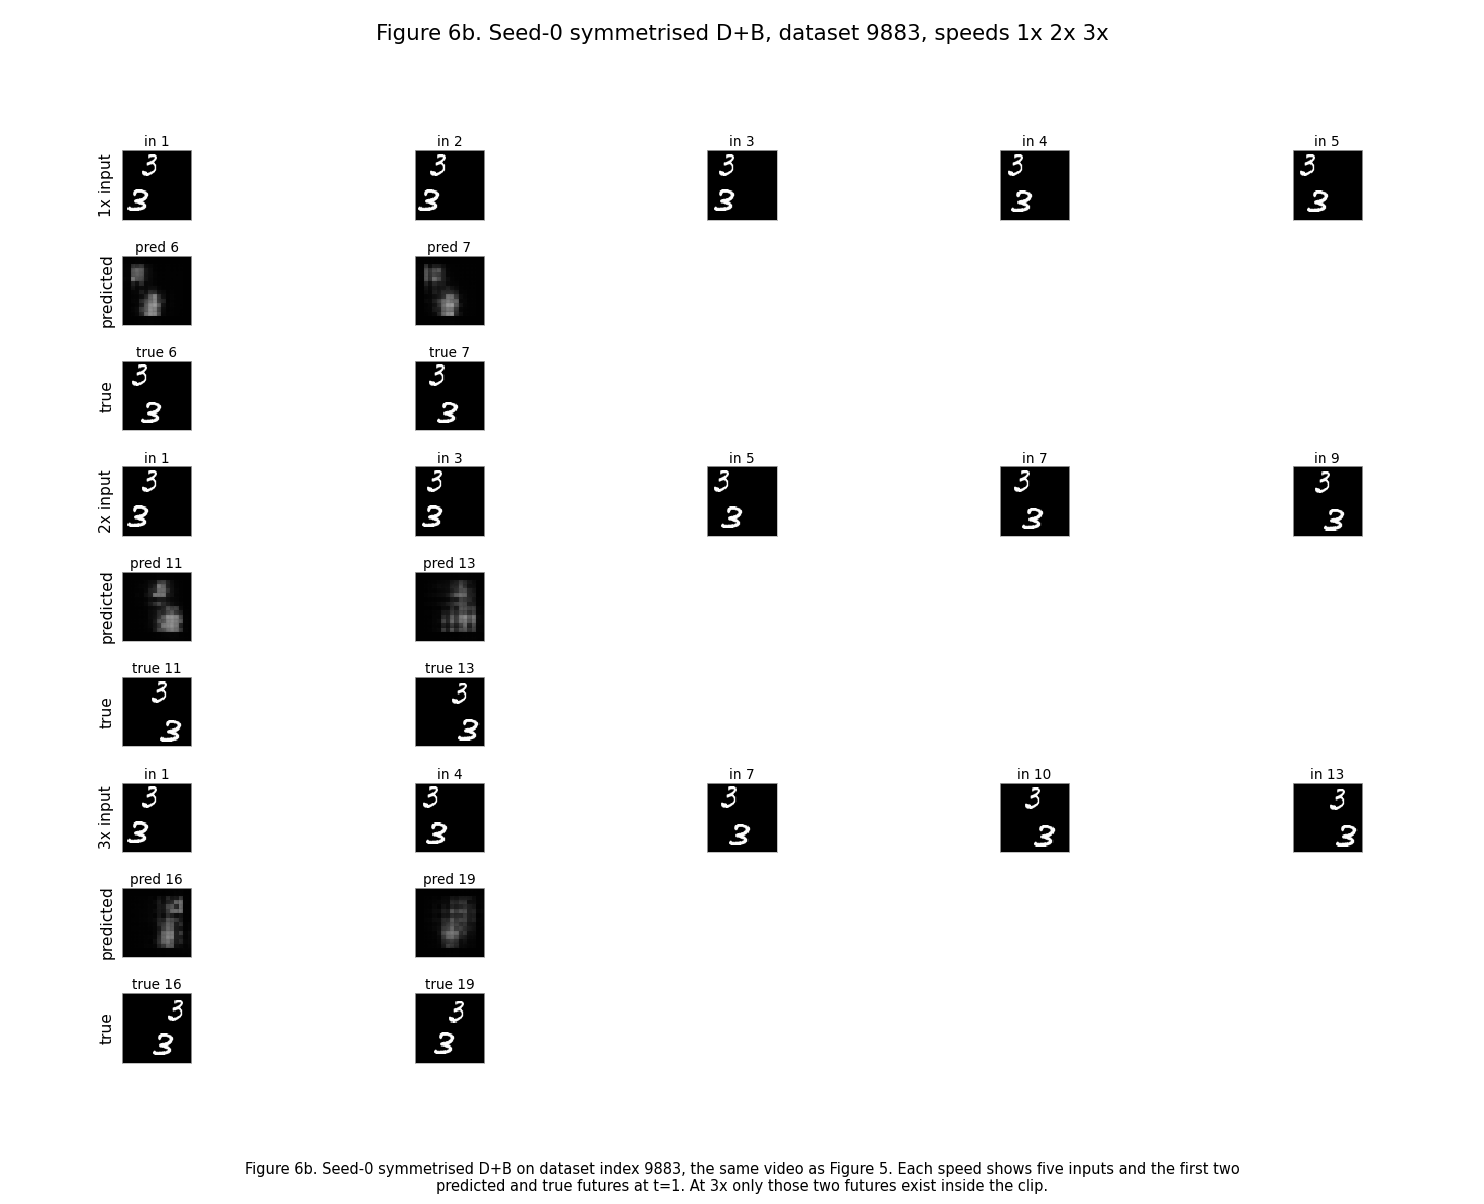
\includegraphics[width=\textwidth]{figure6b.png}
\caption{Figure 6(b). Symmetrised D+B, seed 0, on test video 9883, the same video as Figure~5.}
\end{figure}

\textbf{Q2.15.} Learned symmetry leaves a gap. Built-in symmetry does not. Model B's \(C_M\) is 0.00106 and its \(C_R\) is 0.00132. D+B's are \(7.53\times10^{-4}\) and \(9.89\times10^{-4}\). The wrapped models have gaps of order \(10^{-17}\), and their \(E_M\) and \(E_R\) equal their \(E(5)\). The wrapper is the one that is exact, because the identity above does not depend on the weights. Averaging eight forecasts blurs the frame when those eight put the ink in different places. That did not dominate here. Wrapped B's \(E(5)\) is 0.0218 against learned B's 0.0223, and wrapped D+B's is 0.0281 against learned D+B's 0.0285. The cost is inference. Wrapped B takes 3.81 seconds against learned B's 0.464 seconds. Wrapped D+B takes 4.95 seconds against 0.712 seconds, about seven underlying evaluations.

\textbf{Q2.16.} The video is 9347, the one in Q2.7. The final model removes the disagreement between rows 3 and 4. On seed-0 symmetrised D+B the per-video \(C_M\) is \(7.99\times10^{-17}\), so the two orders are the same image. It does not get horizon 5 right. The truth still has two digits, and the forecast is one blob between them. The wrapper is what made the rows agree. The missing second digit was already missing in the underlying forecast, and an exact symmetry copies that merge into both orders. Dilation and the group augmentation did not keep the two digits apart through horizon 5.

\textbf{Q2.17.}
Symmetrised D+B has mean \(E(2)\) 0.0259 at \(1\times\), 0.0286 at \(2\times\), and 0.0309 at \(3\times\). Model A was 0.0186, 0.0448, and 0.0520. Blank stays near 0.0426, so the wrapped \(2\times\) and \(3\times\) forecast beats an empty frame, and those speeds were in training. On video 9883 the truth keeps two digits. The prediction is one component by frame 7 at \(1\times\) and by frame 11 at \(2\times\). At \(3\times\) the forecast is one blob between the two paths. A skeptic should require both centroids to track the truth on a non-overlapping clip at a speed the training loop never drew. A \(4\times\) window has not been run.

\section*{AI use disclosure}
I used Cursor (Composer) while coding and while drafting this report.

\noindent\textbf{Coding prompts (summary):} set up the repo off Google Drive; run Table 1; check that Model A has 480{,}784 parameters; train on a Kaggle Tesla T4; make the optical-flow figure; design the river model; design Model D; train B, C, D, and D+B; symmetrise the forecaster; write the report.

\noindent\textbf{Model help on code:} wrote \texttt{transforms.py}, \texttt{windows.py}, \texttt{data.py}, \texttt{metrics.py}, \texttt{convlstm.py}, \texttt{model\_a.py}, \texttt{model\_d.py}, and \texttt{symmetrise.py}; wrote the training scripts \texttt{train\_a.py}, \texttt{train\_b.py}, \texttt{train\_c.py}, \texttt{train\_d.py}, and \texttt{train\_db.py}; ran Table 1, Figure 1, and every training and evaluation job on Kaggle (Tesla T4). Model D's dilation and the choice to train D+B were made in that work.

\noindent\textbf{My edits on code:} checked that Table 1 matches, that Model A and Model D each have 480{,}784 parameters, that Q2.5 and Q2.11 were pushed before the experiments they precede, and that every reported test number matches the result JSON files.

\noindent\textbf{Question 1:} Cursor drafted the six headings. The history length and the six-step horizon are assumptions A1 and A2, because the brief leaves both unspecified. I checked that the section separates those assumptions from the given river, and that future rain is not an input while an already announced release is.

\noindent\textbf{Question 2:} Cursor implemented the model, training, and figure scripts and ran them on Kaggle (Tesla T4). I checked Table 1, the 480{,}784 parameter count, and that the reported test numbers come from the result files. Q2.5 was committed as \texttt{10cb5f4} at 14:35 on 27 October 2026, before the mirror, rotation, and speed tests. Q2.11 was committed as \texttt{ede80b4} at 16:20 the same day, before training B, C, and D.

\end{document}
